\documentclass[11pt,a4paper]{article}
\usepackage{amsmath}
\usepackage{amsfonts}
\usepackage{amssymb}
\usepackage{fancyhdr}
\usepackage{lastpage}
\usepackage{graphicx}
\usepackage{ucs}
\usepackage[utf8x]{inputenc}
\usepackage[italian]{babel}
\usepackage[colorlinks=true,linkcolor=black]{hyperref}

\renewcommand{\headrulewidth}{0.6pt}
\renewcommand{\footrulewidth}{0.6pt}
% impostazione dello stile per le pagine interne del documento
\lhead{\leftmark}
\chead{}
\rhead{
\includegraphics[scale=0.15]{logo.png} }
\lfoot{Manuale Utente - Segreteria Didattica v1.0.0}
\cfoot{}
\rfoot{\thepage \ di \pageref{LastPage}}
% ridefinizione dello stile plain per il frontespizio
\fancypagestyle{plain}{
\fancyhf
}
% impostazione dello stile per l'indice
\fancypagestyle{indice}{
\lhead{\leftmark}
\chead{}
\rhead{
\includegraphics[scale=0.15]{logo.png}}
\lfoot{Manuale Utente v1.0.0}
\cfoot{}
\rfoot{}
}
\headheight = 46pt
%definizione del comando "\modfiche" per la creazione del diario delle modifiche
\newcommand{\modifiche} 
{
\newpage
\begin{center}
\textbf{Diario delle modifiche} \\
\bigskip
\begin{tabular}{|c|c|p{0.62\textwidth}|}
\hline
\textsc{Data} & \textsc{Versione} & \textsc{Modifica} \\
\hline
\hline
\textit{15-06-2009} & 1.0.0 & Aggiornamenti vari e approvazione del Responsabile\\
\hline
\textit{06-05-2009} & 0.6.0 & Aggiornati gli screenshot\\
\hline
\textit{03-03-2009} & 0.4.0 & Aggiunto il Glossario\\
\hline
\textit{03-03-2009} & 0.3.1 & Correzioni varie\\
\hline
\textit{02-03-2009} & 0.3.0 & Stesura  della Descrizione funzionale e delle Azioni richieste-permesse\\
\hline
\textit{26-02-2009} & 0.2.0 & Inserite la premessa e le sezioni Introduzione e Descrizione Generale\\
\hline
\textit{24-02-2009} & 0.1.0 & Stesura indice\\
\hline
\end{tabular}
\end{center}
}
%definizione del comando "\info" per la creazione delle informazioni del documento
\newcommand{\info} {
\bigskip
\begin{tabbing}
	\hspace*{0.3\textwidth} \= \hspace*{0.5\textwidth} \kill
	\parbox{0.3\textwidth}{\textbf{Verifica: }} \> \parbox{0.5\textwidth}{Alberti Andrea} \\
	\parbox{0.3\textwidth}{\textbf{Approvazione: }} \> \parbox{0.5\textwidth}{Beggiato Andrea} \\
	\parbox{0.3\textwidth}{\textbf{Stato: }} \> \parbox{0.5\textwidth}{Formale} \\
	\parbox{0.3\textwidth}{\textbf{Uso: }} \> \parbox{0.5\textwidth}{Esterno} \\
	\parbox{0.3\textwidth}{\textbf{Distribuzione: }} \> \parbox{0.5\textwidth}{QuiXoft} \\
							\> \parbox{0.5\textwidth}{Rossi Francesca} \\
							\> \parbox{0.5\textwidth}{Vardanega Tullio} \\
							\> \parbox{0.5\textwidth}{Conte Renato} \\
\end{tabbing}
}
%definizione del comando "\frontespizio" per la creazione del frontespizio
\newcommand{\frontespizio} {
\thispagestyle{plain}
\title{\begin{Huge}\textsc{Progetto SIGEOL}\end{Huge} \\ \textit{Manuale Utente - Segreteria Didattica\\ v1.0.0}}
\author{Redazione: Scortegagna Carlo}
\maketitle
\medskip
\begin{center}

\includegraphics[scale=0.5]{logo.png} \\
\textit{quixoft.sol@gmail.com} \\
\end{center}
\medskip
\info
\begin{center}
\textbf{Sommario} \\
Manuale utente per l'utilizzo del progetto \textit{SIGEOL} da parte della segreteria didattica, contenente la spiegazione di tutte le funzionalità disponibili, dei possibili problemi e delle relative soluzioni.
\end{center}
\newpage
}
%definizione del comando "\indice" per la creazione dell'indice
\newcommand{\indice} {
\thispagestyle{indice}
\tableofcontents
\newpage
}
\pagestyle{fancy}
\begin{document}
\frontespizio
\indice
\setcounter{page}{1}
\section{Premessa}
L'utilizzo del progetto software SIGEOL è previsto da 3 differenti tipologie d'utenti:
\begin{enumerate}
 \item Utenti che non abbiano effettuato il \underline{login} (in seguito riferiti come visitatori) che accedono al sistema solo per consultare informazioni
 \item Docenti che abbiano accreditato la propria identità tramite login
 \item Segreteria Didattica che accede al sistema tramite login
\end{enumerate}
\bigskip
Le funzionalità offerte ai visitatori sono solamente di consultazione di informazioni: possono consultare lo schema d'orario dei diversi corsi di laurea, possono accedere alle informazioni relative ai docenti, alle aule, agli edifici, agli insegnamenti, ecc...

Dato il largo numero di utenti visitatori che accederanno al progetto SIGEOL, la diffusione di un eventuale manuale utente dedicato a loro risulterebbe piuttosto scomoda.

Le operazioni dedicate solamente ai visitatori saranno quindi ampiamente commentate e descritte proprio all'interno dell'interfaccia grafica, per facilitare la consultazione delle varie informazioni ai visitatori senza che questi debbano leggere un eventuale manuale utente.

\bigskip \bigskip
Data la gran diversità delle operazioni accessibili dalle due rimanenti tipologie d'utenza, saranno redatti due distinti manuali utente: i docenti dovranno consultare il documento \textsc{Manuale Utente Docente}, la segreteria didattica invece dovrà consultare il \textsc{Manuale Utente Segreteria Didattica}.

Caso particolare a quanto appena affermato è il Presidente del CCS: avendo a disposizione sia le funzioni dedicate ai docenti sia quelle dedicate alla segreteria didattica, per questo utente del sistema SIGEOL è consigliata la consultazione di entrambi i manuali.
\newpage
\section{Introduzione}
\subsection{Definizione dell'utente del prodotto}
Il presente manuale utente è rivolto alla spiegazione delle diverse funzionalità del sistema SIGEOL dedicate all'utenza denominata segreteria didattica.
L'accesso alle operazioni descritte in seguito è possibile solamente dopo aver effettuato con successo il login al sistema, confermando di avere i privilegi assegnati all'utente segreteria didattica.

Sia prima sia dopo aver effettuato il login, sono sempre disponibili anche le funzioni di consultazione informazioni dedicate agli utenti visitatori, ampiamente descritte all'interno dell'interfaccia grafica, e quindi non illustrate nel presente documento.
\subsection{Come leggere il manuale}
Il presente manuale descrive brevemente le parti pubbliche del progetto (vedi sezione `Descrizione Generale`) e si focalizza in seguito sulle funzionalità private dedicate alla segreteria didattica (sezione `Azioni Richieste - Permesse`).

Saranno illustrate e descritte tutte le possibili operazioni effettuabili, con l'aiuto di \underline{screenshot} qualora ve ne fosse la necessità.

Proseguendo con la lettura, saranno elencati i vari errori a cui si potrà andare incontro utilizzando il progetto SIGEOL, e le eventuali soluzioni per porvi rimedio.

Il manuale termina con un Glossario, contenente la spiegazione di alcuni termini usati nel corso di questo documento.
I termini che possiedono una descrizione all'interno del Glossario saranno riconoscibili perchè presentano una \underline{sottolineatura}.

\subsection{Come riportare problemi e malfunzionamenti}
La segnalazione di problemi o manfulzionamenti del sistema SIGEOL andrà fatta inviando un email all'indirizzo \textit{quixoft.sol@gmail.com}.
Quest'ultima dovrà contenere le seguenti informazioni:
\begin{itemize}
 \item Nome e cognome del mittente
 \item Data e ora in cui il problema si è manifestato
 \item Tipo d'utenza
 \item Informazioni sull'ambiente in cui è stato rilevato l'errore (sistema operativo, \underline{browser}, ecc...) o qualsiasi altra informazione d'utilità ritenuta importante dal mittente (configurazione hardware, risoluzione dello schermo, ecc...)
 \item Descrizione del malfunzionamento riscontrato, dei messaggi d'errore visualizzati, delle eventuali operazioni svolte prima del manifestarsi del problema.
\end{itemize}
Le segnalazioni saranno prese in considerazione il prima possibile e i problemi riscontrati saranno risolti al più presto dai membri del team QuiXoft.
\section{Descrizione generale}
Il progetto SIGEOL si presenta all'utente come un semplice sito internet, la cui consultazione è similare e non presenta difficoltà rispetto ai canoni classici delle pagine che compongono il \underline{World Wide Web}.

Tale sito è raggiungibile utilizzando un qualsiasi elaboratore connesso ad internet: l'unico software necessario per la sua consultazione è un semplice browser (come, ad esempio, Firefox, Internet Explorer, Chrome, Safari, Opera, ecc...).

L'effettivo indirizzo internet a cui raggiungere il sito del progetto SIGEOL non è al momento noto con certezza e non verrà di conseguenza menzionato nel presente documento: sarà compito del Committente scegliere e predisporre tale indirizzo.

Una volta digitato l'indirizzo internet corretto nel browser sarà visualizzata la pagina principale del progetto, contenente le prime informazioni e i \underline{link} alle altre pagine disponibili.

Prima di effettuare il login saranno disponibili e visualizzate solamente le pagine pubbliche, che consentono di consultare:
\begin{itemize}
 \item orari di lezione per i vari corsi di laurea presenti
 \item informazioni riguardanti i suddetti corsi di laurea e gli insegnamenti
 \item informazioni personali e contatti dei docenti assegnati ai vari insegnamenti
 \item informazioni sugli edifici e sulle aule presenti
\end{itemize}
Sarà inoltre possibile generare un file in formato \underline{Pdf} con l'orario richiesto, per poterlo facilmente stampare o salvare localmente.

Come detto in precedenza, le funzioni appena elencate sono di immediato utilizzo e non verrano quindi spiegate esaustivamente nel presente documento.
Una semplice spiegazione del loro funzionamento sarà presente direttamente all'interno delle relative pagine del sito web del progetto.

\bigskip
Una volta effettuato il login con l'indirizzo email e la password assegnati alla segreteria didattica, saranno disponibili anche tutte le funzioni di amministrazione del sito:
\begin{itemize}
 \item Inserimento di un nuovo corso di laurea, dei vari curriculum e dei relativi vincoli
 \item Inserimento degli edifici e delle aule messe a disposizione, con i relativi vincoli
 \item Inserimento degli insegnamenti e assegnazione ai relativi docenti
 \item Invito e gestione dei docenti
 \item Generazione dell'orario
 \item Cambio password del proprio \underline{account}
\end{itemize}
Le funzioni appena elencate saranno accuratamente illustrate nel proseguire del presente documento.
\subsection{Interfaccia grafica}
L'aspetto grafico del sito internet è pensato per essere il più semplice ed intuitivo possibile. Potrà però accadere che il committente, a seguito dell'accettazione del prodotto, richieda delle modifiche superficiali al layout o all'aspetto grafico delle pagine (colori, caratteri, ecc...), per adeguarsi allo stile delle pagine internet già in suo possesso o per adattarsi ai suoi gusti.

Il \underline{template} attuale è da ritenersi passibile di variazioni e, di conseguenza, le immagini consultabili all'interno del presente documento potranno non rappresentare esattamente l'aspetto reale del sito Internet. Le possibile modifiche saranno comunque solamente estetiche: le funzionalità e i dati da inserire saranno identici.
\section{Istruzioni per l'uso}
\subsection{Descrizione funzionale}
\subsubsection{Pagina Principale}
La pagina principale del prodotto SIGEOL mostra gli orari delle lezioni per tutti i corsi di laurea gestiti dal sistema, raggruppati per anno e per periodo. E' possibile consultare tali orari via browser oppure è possibile generare un file in formato Pdf per il salvataggio o per la stampa.

Seguendo i link presenti in alto sotto il titolo, è possibile consultare tutte le informazioni pubbliche. E' possibile visualizzare le informazioni relative a:
\begin{itemize}
 \item Docenti registrati al sistema e relativi dati personali (link 'Docenti')
 \item Edifici e aule gestiti dal sistema, con indirizzi e mappe per raggiungerli (link 'Strutture')
 \item Insegnamenti gestiti, divisi per corso di laurea (link 'Insegnamenti')
\end{itemize}

E' inoltre sempre possibile ritornare alla pagina principale di consultazione degli orari seguendo il link 'Home'.

Sul lato sinistro del sito si trova la form di login, in cui si potranno inserire il proprio indirizzo email e la propria password per accedere alle aree e alle funzioni private riservate ai docenti.
\subsection{Azioni richieste/permesse}
Ogni capitolo di questa sezione si riferisce ad una particolare funzione che il sistema SIGEOL mette a disposizione dell'utente segreteria didattica. Tali funzioni sono raggiungibili da un link presente nella barra laterale, sul lato sinistro del sito, dopo aver effettuato correttamente il login come illustrato nella seguente sezione.
\subsubsection{Form di Login}
La form di login, come si vede in figura 4.2.1.1, offre la possibiltà agli utenti come la segreteria didattica o i docenti di inserire il proprio username (corrispondente all'indirizzo email) e la relativa password per poter accedere alle funzioni private messe a loro disposizione.

\bigskip
\begin{center}
	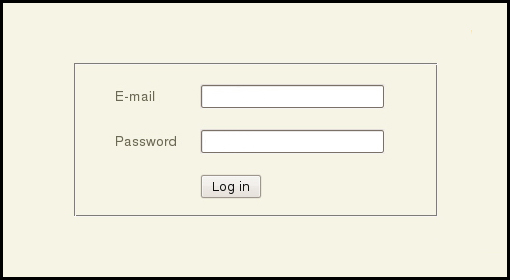
\includegraphics[scale=0.5]{images/login.jpg}\\
	\textbf{fig. 4.2.1.1} Form di login\\
\end{center}
\bigskip

In caso di login corretto verrà visualizzata nuovamente la pagina principale del prodotto SIGEOL, con in più i link a tutte le funzioni private accessibili.
In caso di errore nell'inserimento dell'indirizzo email o della password verrà visualizzato un messaggio di notifica di tale errore.
Sarà immediatamente possibile reinserire i dati corretti e ritentare il login.

Le funzioni accessibili alle due tipologie di utenti appena citate sono diametralmente opposte: nei successivi capitoli del presente documento verranno quindi solamente illustrate le funzioni dedicate alla segreteria didattica.
\subsubsection{Gestione Corsi di Laurea}
La pagina di gestione dei corsi di laurea, raggiungibile seguendo il link `Corsi di laurea` presente nella barra laterale, mostra una lista di tutti i corsi inseriti dalla segreteria didattica e dei relativi curricula. Una sua anteprima d'esempio è visibile in figura 4.2.2.1.

\bigskip
\begin{center}
	%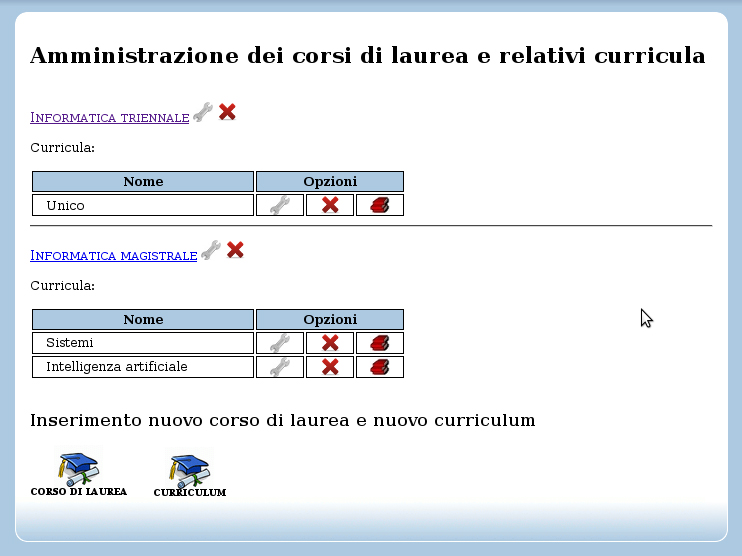
\includegraphics[scale=0.5]{images/corsi_di_laurea.jpg}\\
	\textbf{fig. 4.2.1.1} Pagina di Gestione dei corsi di laurea\\
\end{center}
\bigskip

Da questa pagina amministrativa è possibile:
\begin{itemize}
 \item visualizzare le informazioni relative a quel corso di laurea cliccando sul suo nome.
 \item modificare i suoi dati seguendo il link `Modifica i dati`, caratterizzato dall'icona a forma di chiave inglese
 \item eliminare quel determinato corso di laurea seguendo il link `Elimina definitivamente dal sistema`, caratterizzato dall'icona a forma di X rossa. Una finestra di popup chiederà conferma di tale azione. Prestare attenzione al fatto che tutti i curriculum e tutti gli insegnamenti legati al corso di laurea che ci si presta a cancellare verranno definitivamente eliminati dal sistema, senza possibilità di ripristino.
\end{itemize}

Per ogni corso di laurea sono elencati tutti curricula che ne fanno parte.
Per ogni curriculum è possibile:
\begin{itemize}
 \item modificare i dati del curriculum seguendo il link `Modifica i dati`, caratterizzato dall'icona a forma di chiave inglese
 \item eliminare quel determinato curriculum seguendo il link `Elimina definitivamente dal sistema`, caratterizzato dall'icona a forma di X rossa. Una finestra di popup chiederà conferma di tale azione. Prestare attenzione al fatto che tutti gli insegnamenti legati al curriculum che ci si presta a cancellare verranno definitivamente eliminati dal sistema, senza possibilità di ripristino.
 \item gestire gli insegnamenti che appartengono a quel curriculum seguendo il link `Gestisci gli insegnamenti`, caratterizzato dall'icona con i libri, la terza partendo da destra nella tabella.
\end{itemize}

Verranno qui di seguito descritte in dettaglio le funzionalità di inserimento dei corsi di laurea, di inserimento e di modifica dei curriculum e la pagine di gestione degli insegnamenti per i curricula:
\newline \newline
\begin{large}\textbf{Inserimento di un nuovo corso di laurea:}\end{large}

\bigskip
\begin{center}
	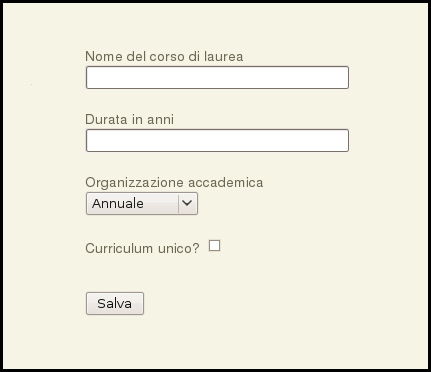
\includegraphics[scale=0.5]{images/nuovo_corso.jpg}\\
	\textbf{fig. 4.2.1.1} Form di inserimento di un corso di laurea\\
\end{center}
\bigskip

Seguendo il link `Inserisci un nuovo corso di laurea` si accede alla pagina visibile in figura 4.2.1.1, la quale richiede:
\begin{itemize}
 \item inserimento del nome del corso di laurea: il nome non deve essere vuoto e deve contenere solamente caratteri o spazi. Sono vietati numeri o simboli. La lunghezza massima è fissata in 50 caratteri, compresi gli spazi.
 \item inserimento della durata in anni: deve essere inserito un numero compreso tra 1 e 6.
 \item scelta dell'organizzazione accademica: la scelta deve essere fatta tramite menu a tendina tra le varie opzioni proposte, che al momento sono annuale, semestri, trimenstri, quadrimestri. Serve a determinare in quanti periodi è suddiviso l'anno di quel determinato corso di laurea.
 \item nel caso il corso di laurea che si sta inserendo preveda un solo curriculum, è necessario selezionare la casella `Curriculum Unico`. Nel caso il corso di laurea preveda più curriculum, è sufficiente non selezionare tale opzione e inserire i vari curriculum successivamente. La scelta non è vincolante: è possibile eliminare o aggiungere curriculum a piacimento successivamente alla creazione del corso di laurea.
\end{itemize}
Al termine dell'inserimento dei dati richiesti, sarà sufficiente premere il bottone `Crea` per salvare il nuovo corso di laurea.

Se si è selezionato `Curriculum unico` verrà di seguito visualizzata nuovamente la pagina principale di gestione dei corsi di laurea.
Se invece non è stato selezionato `Curriculum unico` verrà visualizzata la pagina di creazione di un nuovo curriculum, descritta in seguito.
\newline \newline
\begin{large}\textbf{Inserimento di un nuovo curriculum:}\end{large}

\bigskip
\begin{center}
	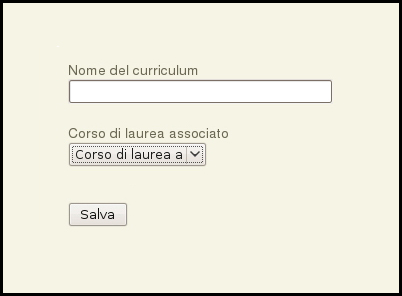
\includegraphics[scale=0.5]{images/nuovo_curriculum.jpg}\\
	\textbf{fig. 4.2.1.3} Form di inserimento di un curriculum\\
\end{center}
\bigskip

Seguendo il link `Inserisci un nuovo curriculum` si accede alla pagina visibile in figura 4.2.1.3, la quale richiede:
\begin{itemize}
 \item inserimento del nome del curriculum: deve contenere solo caratteri o spazi e la sua lunghezza massima è fissata in 50 caratteri
 \item scelta del corso di laurea di cui il curriculum fa parte, tramite menu a tendina
\end{itemize}
Premendo il bottone `Crea` verrà salvato il curriculum e si verrà reindirizzati alla pagina di gestione dei corsi di laurea. Il nuovo curriculum appena creato sarà presente nella lista del relativo corso di laurea.
\newline \newline
\begin{large}\textbf{Modifica dei dati di un curriculum:}\end{large}

\bigskip
\begin{center}
	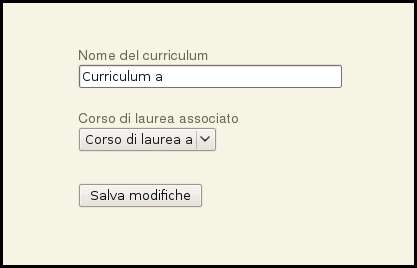
\includegraphics[scale=0.5]{images/modifica_curriculum.jpg}\\
	\textbf{fig. 4.2.1.4} Form di modifica di un curriculum\\
\end{center}
\bigskip

La pagina per modificare i dati di un curriculum esistente, visibile in figura 4.2.1.4, funziona in modo similare alla pagina di inserimento appena illustrata. I campi che è possibile modificare sono infatti:
\begin{itemize}
 \item nome del curriculum
 \item scelta del corso di laurea di cui il curriculum fa parte, tramite menu a tendina
\end{itemize}
Le regole da seguire per la loro compilazione sono identiche a quelle sopra illustrate per l'inserimento di un nuovo curriculum.
\newline \newline
\begin{large}\textbf{Gestione degli insegnamenti:}\end{large}

\bigskip
\begin{center}
	%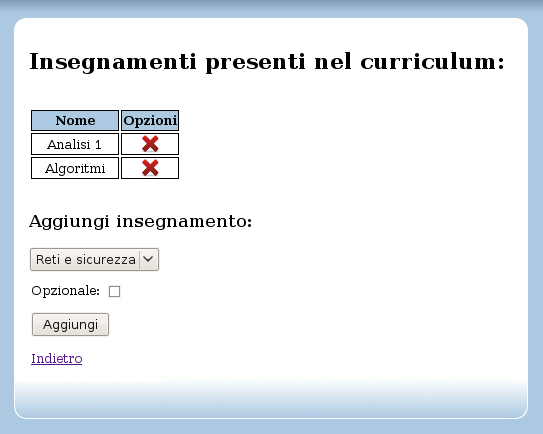
\includegraphics[scale=0.5]{images/gestisci_insegnamenti.jpg}\\
	\textbf{fig. 4.2.2.5} Pagina di gestione degli insegnamenti\\
\end{center}
\bigskip

Seguendo il link `Gestisci gli insegnamenti`, è a disposizione una pagina in cui sono elencati tutti gli insegnamenti assegnati a quel particolare curriculum, come visibile in figura 4.2.2.5.

E' data la possibilità di rimuovere uno o più insegnamenti dal curriculum seguendo il link `Rimuovi l'insegnamento dal curriculum`, caratterizzato dall'icona a forma di X rossa.
E' possibile anche aggiungere un insegnamento al curriculum selezionandolo dal menu a tendina e premendo il bottone `Aggiungi`.
Queste due funzioni sono particolarmente utili per corsi di laurea che prevedono curriculum multipli, in quanto due o più curriculum all'interno dello stesso corso di laurea potrebbero condividere un particolare insegnamento.

\subsubsection{Gestione Edifici}
La pagina di gestione degli edifici, come visibile in figura 4.2.3.1, contiene una lista di tutti gli edifici a disposizione dalla segreteria didattica.
E' possibile:
\begin{itemize}
 \item consultare le informazioni relative ad un determinato edificio cliccando sul suo nome
 \item modificare i suoi dati seguendo il link `Modifica i dati`, caratterizzato dall'icona a forma di chiave inglese
 \item eliminare quel determinato edificio seguendo il link `Elimina definitivamente dal sistema`, caratterizzato dall'icona a forma di X rossa. Una finestra di popup chiederà conferma di tale azione. Prestare attenzione al fatto che tutte le aule presenti all'interno dell'edificio che ci si presta a cancellare verranno definitivamente eliminati dal sistema, senza possibilità di ripristino.
\end{itemize}

\bigskip
\begin{center}
	%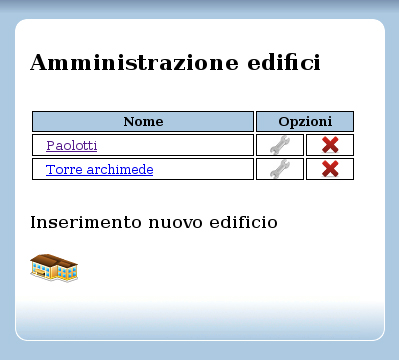
\includegraphics[scale=0.5]{images/amministrazione_edifici.jpg}\\
	\textbf{fig. 4.2.2.5} Pagina di gestione degli edifici\\
\end{center}
\bigskip

E' importante ricordarsi di creare gli edifici necessari prima di creare una o più aule che sono presenti all'interno di quella struttura. In caso contrario, la nuova aula creata non potrà essere assegnata al corretto edificio.

Le funzioni di inserimento di un nuovo edificio e di modifica dei dati di un edificio già presente sono illustrate più in dettaglio qui di seguito:
\newline \newline
\begin{large}\textbf{Inserimento di un nuovo edificio:}\end{large}
\\ \\
\begin{center}
	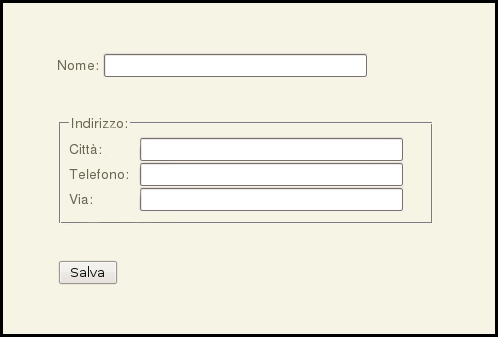
\includegraphics[scale=0.5]{images/nuovo_edificio.jpg}\\
	\textbf{fig. 4.2.2.1} Form di inserimento di un edificio\\
\end{center}
\bigskip

La pagina di inserimento di un nuovo edificio, come illustrato in figura 4.2.2.1, richiede l'inserimento obbligatorio dei seguenti dati:
\begin{itemize}
 \item nome dell'edificio: deve essere composto solamente da caratteri, numeri e spazi. La lunghezza massima del nome è stata fissata in 30 caratteri.
 \item città: il nome della città in cui si trova l'edificio deve essere composto solamente da caratteri o spazi. Anche in questo caso la lunghezza massima è fissata in 30 caratteri.
 \item numero di telefono: deve essere inserito nel formato `prefisso-numero`. Il prefisso può essere composto solamente da numeri e la sua lunghezza può variare da 2 a 4. Anche il numero segue le stesse regole, ma la lunghezza dev'essere compresa tra 6 e 8 cifre.
 \item via: si accettano caratteri, numeri e spazi. In questo caso la lunghezza massima è fissata in 50 caratteri, compresi gli spazi.
\end{itemize}
Al termine dell'inserimento di tutti i dati richiesti è sufficiente premere sul pulsante `Crea` per salvare l'edificio e il relativo indirizzo nel sistema SIGEOL.
Da questo momento è possibile inserire delle aule all'interno dell'edificio appena salvato.
\newline \newline
\begin{large}\textbf{Modifica dei dati di un edificio:}\end{large}

\bigskip
\begin{center}
	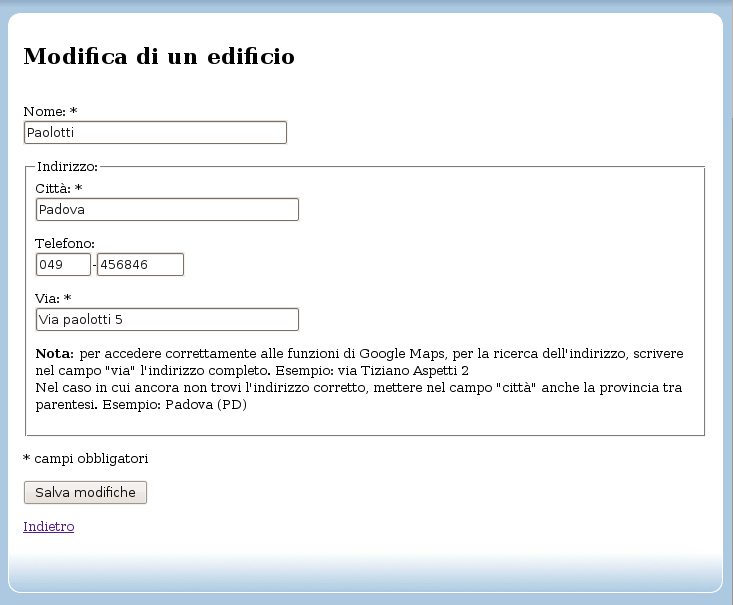
\includegraphics[scale=0.5]{images/modifica_edificio.jpg}\\
	\textbf{fig. 4.2.2.2} Form di modifica di un edificio\\
\end{center}
\bigskip

Come visualizzato in figura 4.2.2.2, la pagina di modifica dei dati di un edificio già presente nel sistema SIGEOL è di funzionamento simile alla pagina di inserimento appena descritta. Si possono modificare gli stessi dati inseriti in fase di creazione dell'edificio e le regole da rispettare per la modifica delle varie informazioni sono le stesse sopra elencate.

Al termine delle modifiche è sufficiente premere il bottone `Salva modifiche` per salvare le modifiche nel sistema SIGEOL.
\subsubsection{Gestione Aule}
La pagina di gestione delle aule contiene, in modo simile a tutte le altre pagine di amministrazione disponibili per la segreteria didattica, una lista delle aule a diposizione, raggruppate per edificio.
E' possibile:
\begin{itemize}
 \item consultare le informazioni relative ad una data aula cliccando sul link presente sul suo nome.
 \item modificare i suoi dati seguendo il link `Modifica i dati`, caratterizzato dall'icona a forma di chiave inglese
 \item gestire i vincoli temporali di indisponibilità dell'aula seguendo il link `Gestisci le disponibilità e le prenotazioni`, caratterizzato dall'icona a forma di orologio.
 \item eliminare quella determinata aula seguendo il link `Elimina definitivamente dal sistema`, caratterizzato dall'icona a forma di X rossa. Una finestra di popup chiederà conferma di tale azione. Tale azione non ha possibilità di essere annullata.
\end{itemize}

\bigskip
\begin{center}
	%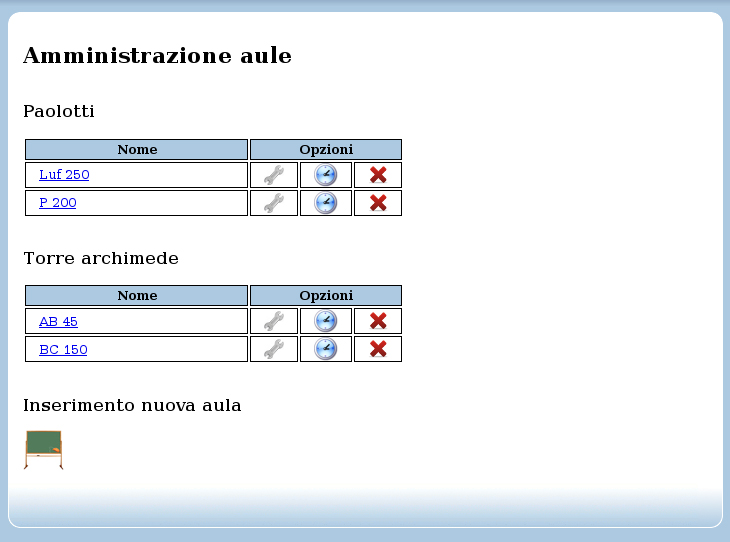
\includegraphics[scale=0.5]{images/amministrazione_aule.jpg}\\
	\textbf{fig. 4.2.2.5} Pagina di gestione delle aule\\
\end{center}
\bigskip

Le funzionalità di inserimento di una nuova aula, di modifica dei dati di una già presente e di gestione dei vincoli sono illustrate in maggior dettaglio qui di seguito:
\newline \newline
\begin{large}\textbf{Inserimento di una nuova aula:}\end{large}

\bigskip
\begin{center}
	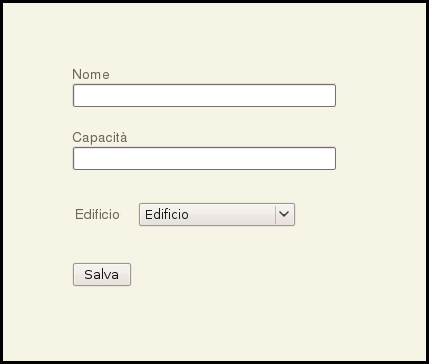
\includegraphics[scale=0.5]{images/nuova_aula.jpg}\\
	\textbf{fig. 4.2.3.1} Form di inserimento di un'aula\\
\end{center}
\bigskip

La pagina di inserimento di una nuova aula, come visualizzato in figura 4.2.3.1, richiede i seguenti dati:
\begin{itemize}
 \item nome dell'aula: deve essere non vuoto, può solamente contenere caratteri, numeri o spazi; la lunghezza massima è fissata in 30 caratteri. 
 \item capacità dell'aula: deve essere un numero intero compreso tra 1 e 1000
 \item laboratorio: spuntare la casella nel caso l'aula che si sta inserendo sia un laboratorio. Nel calcolo dell'orario solamente le ore di lezione di laboratorio potranno essere assegnate a quest'aula.
 \item scelta dell'edificio in cui l'aula è ubicata, tramite menu a tendina. Nel caso l'edificio non fosse ancora presente nel sistema SIGEOL, è necessario, prima della fase di creazione dell'aula, inserire i dati dell'edificio: per maggiori informazioni si prega di consultare la sezione `Inserimento di un nuovo edificio`.
\end{itemize}
Una volta inseriti correttamente tutti i dati è sufficiente premere il pulsante `Crea` per salvare la nuova aula.

Da notare che l'aula viene messa automaticamente a disposizione di tutti i corsi di laurea presenti nel sistema SIGEOL: se tale scelta non fosse corretta, sarà necessario passare alla fase di modifica dei dati dell'aula.
\newline \newline
\begin{large}\textbf{Modifica dei dati di un aula:}\end{large}

\bigskip
\begin{center}
	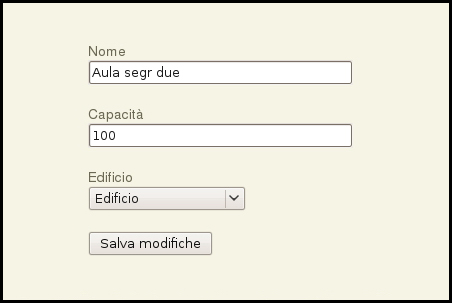
\includegraphics[scale=0.5]{images/modifica_aula.jpg}\\
	\textbf{fig. 4.2.3.2} Form di modifica di un aula\\
\end{center}
\bigskip

Come visualizzato in figura 4.2.3.2, la pagina di modifica dei dati di un aula già presente all'interno del sistema SIGEOL permette di aggiornare i seguenti dati:
\begin{itemize}
 \item nome dell'aula
 \item capacità dell'aula
 \item edificio in cui l'aula è ubicata, tramite menu a tendina
\end{itemize}
Le regole da rispettare per l'inserimento di questi dati sono le stesse sopra illustrate per la fase di inserimento di una nuova aula.
Premendo il bottone `Salva modifiche` i nuovi dati aggiornati saranno salvati nel sistema.

\bigskip
\begin{center}
	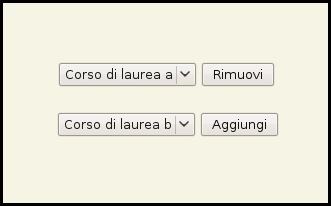
\includegraphics[scale=0.5]{images/modifica_aula_corso.jpg}\\
	\textbf{fig. 4.2.3.3} Form di aggiunta e rimozione delle disponibilità\\
\end{center}
\bigskip

Oltre ai campi appena illustrati, la pagina di modifica dei dati di un aula contiene una lista dei corsi di laurea per i quali quest'aula è messa a disposizione, come visibile in figura 4.2.3.3.
Sarà possibile eliminare la disponibilità dell'aula per un particolare corso di laurea seguendo il link `Rimuovi il corso di laurea dalla lista`, caratterizzato dall'icona a forma di - rosso, presente a fianco di ogni corso di laurea.
Sono di seguito elencati i corsi di laurea per il quali l'aula è stata dichiarata non disponibile: per aggiungere l'aula anche a questi ultimi e sufficienete seguire il link `Aggiungi il corso di laurea alla lista`, caratterizzato dall'icona a forma di + verde, presente a fianco di ogni corso di laurea.

Nel caso vengano rimosse tutte le disponibilità, l'aula non è a disposizione di nessun corso di laurea, e pertanto non verrà mai considerata nella generazione degli orari di lezione.
E' pur sempre possibile rendere nuovamente disponibile quest'aula per qualche corso di laurea in seguito.
\newline \newline
\begin{large}\textbf{Gestione dei vincoli temporali di indisponibilità dell'aula:}\end{large}

\bigskip
\begin{center}
	%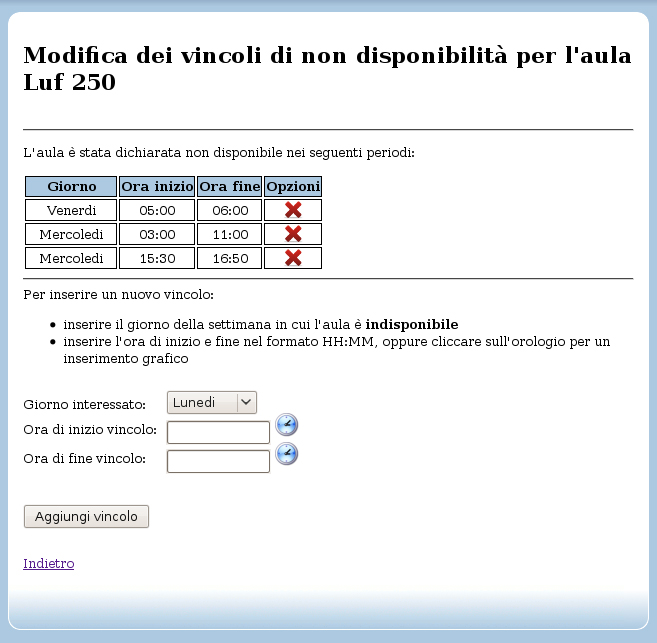
\includegraphics[scale=0.5]{images/gestione_vincoli_aula.jpg}\\
	\textbf{fig. 4.2.3.4} Pagina di gestione dei vincoli di indisponibilità dell'aula\\
\end{center}
\bigskip

Come visualizzato in figura 4.2.3.4, la pagina di gestione dei vincoli temporali di indisponibilità di un aula permette di inserire degli intervalli temporali in cui un aula non è disponibile per ospitare una lezione.
Essa contiene una lista dei vincoli inseriti precedentemente, che potranno essere eventualmente cancellati selezionando il link caratterizzato dalla X rossa, presente a fianco di ogni vincolo.

La pagina dà inoltre la possibilità di inserire un nuovo vincolo di indisponibilità.
I vincoli inseriti all'interno del sistema SIGEOL verranno automaticamente accettati e categoricamente rispettati nel calcolo dell'orario delle lezioni.
Nel caso il sistema non riesca a generare l'orario delle lezioni rispettando tutti i vincoli inseriti, sarà compito della segreteria didattica o del presidente del CCS rilassare uno o più vincoli.

I campi dato da completare nel momento dell'inserimento di un nuovo vincolo sono:
\begin{itemize}
 \item scelta del giorno della settimana, tramite menu a tendina.
 \item scelta dell'intervallo orario: andranno scelti un orario di inizio o un orario di fine del periodo di indisponibilità. E' possibile sia l'inserimento manuale (in tal caso l'orario va inserito nel formato HH:MM) sia l'inserimento grafico, cliccando sull'icona dell'orologio.
\end{itemize}
Al termine dell'inserimento di tutti i dati è sufficiente premere il pulsante `Aggiungi vincolo` per memorizzare il vincolo all'interno del sistema SIGEOL: d'ora in poi tale vincolo verrà rispettato nel calcolo dell'orario delle lezioni.
\subsubsection{Gestione Insegnamenti}
La pagina di gestione degli insegnamenti, come visibile in figura 4.2.5.1, mostra un elenco degli insegnamenti presenti all'interno del sistema SIGEOL, raggruppati per corso di laurea.

\bigskip
\begin{center}
	%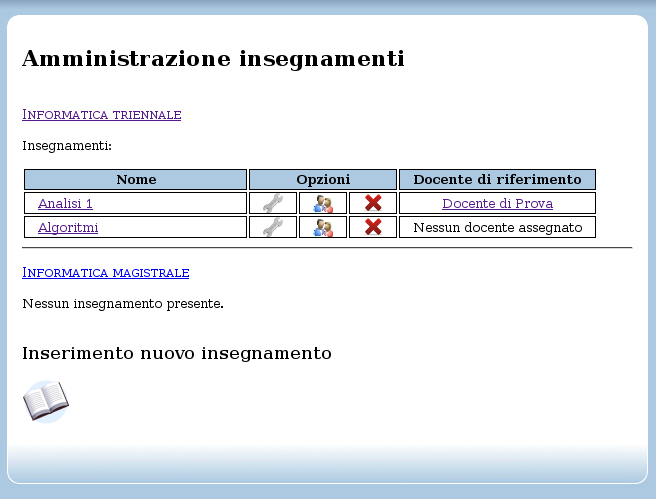
\includegraphics[scale=0.5]{images/amministrazione_insegnamenti.jpg}\\
	\textbf{fig. 4.2.5.1} Pagina di amministrazione degli insegnamenti\\
\end{center}
\bigskip

Come per ogni altra pagina dedicata alla segreteria didattica, è possibile:
\begin{itemize}
 \item consultare le informazioni relative ad un insegnamento cliccando sul link presente sul suo nome.
 \item modificare i suoi dati seguendo il link `Modifica i dati`, caratterizzato dall'icona a forma di chiave inglese
 \item assegnare un docente a quell'insegnamento seguendo il link `Assegna docente di riferimento`, caratterizzato dalla seconda icona partendo da sinistra. E' possibile assegnare un solo docente per ogni corso: nel caso ci sia già un docente assegnato, il seguire questo link permette di assegnare l'insegnamento ad un nuovo docente e contemporaneamente di liberare il vecchio docente assegnato dal suo incarico.
 \item eliminare quell'insegnamento seguendo il link `Elimina definitivamente`, caratterizzato dall'icona a forma di X rossa. Una finestra di popup chiederà conferma di tale azione. Tale azione non ha possibilità di essere annullata.
\end{itemize}

Se un insegnamento presente in lista ha già un docente assegnato, sarà visualizzato il nome di tale docente.
In caso contrario sarà necessario assegnare un docente. Da notare che il docente deve essere preventivamente invitato e registrato al sistema SIGEOL, altrimenti non sarà possibile assegnargli l'insegnamento.

Le funzioni di inserimento di un nuovo insegnamento e di modifica dei dati di uno già presente nel sistema saranno illustrate nel dettaglio qui di seguito:
\newline \newline
\begin{large}\textbf{Inserimento di un nuovo insegnamento:}\end{large}

\bigskip
\begin{center}
	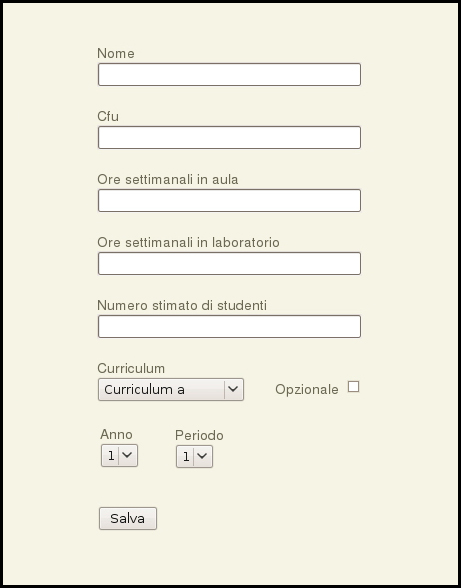
\includegraphics[scale=0.5]{images/nuovo_insegnamento.jpg}\\
	\textbf{fig. 4.2.4.1} Form di inserimento di un insegnamento\\
\end{center}
\bigskip

La pagina di inserimento di un nuovo insegnamento, come illustrato in figura 4.2.4.1, richiede obbligatoriamente i seguenti dati:
\begin{itemize}
 \item nome dell'insegnamento: deve essere composto solamente da caratteri, numeri o spazi; non può essere vuoto e la sua lunghezza massima è fissata in 30 caratteri.
 \item CFU: il numero dei crediti deve essere compreso tra 1 e 20
 \item ore di lezione settimanali in aula: deve essere un numero compreso tra 0 e 40
 \item ore di lezione settimanali in laboratorio: deve essere un numero compreso tra 0 e 40
 \item numero stimato di studenti: deve essere inserito un numero compreso tra 0 e 1000
 \item scelta del curriculum a cui l'insegnamento si riferisce, tramite menu a tendina
 \item scelta dell'anno in cui il corso verrà tenuto nel curriculum selezionato, tramite menu a tendina
 \item periodo in cui il corso verrà tenuto: la scelta verrà fatta tramite menu a tendina e dovrà tener conto dell'organizzazione accademica del corso di laurea su cui si sta agendo.
\end{itemize}
Una volta inseriti tutti i dati, l'insegnamento verrà salvato nel sistema SIGEOL premendo il pulsante `Crea`.
\newline \newline
\begin{large}\textbf{Modifica dei dati di un insegnamento:}\end{large}
\\ \\
La pagina di modifica di un insegnamento già presente all'interno del sistema SIGEOL permette di aggiornare tutti i dati, mantenendo l'aspetto e i campi dato della pagina di inserimento di un nuovo insegnamento.
\subsubsection{Gestione Docenti}
La pagina di gestione dei docenti, come visibile in figura 4.2.6.1, offre innanzitutto una lista dei docenti che sono stati invitati al sistema SIGEOL ma che non hanno ancora completato la registrazione: questi docenti potranno essere gestiti e assegnati ai vari insegnamenti appena completeranno la loro registrazione.

\bigskip
\begin{center}
	%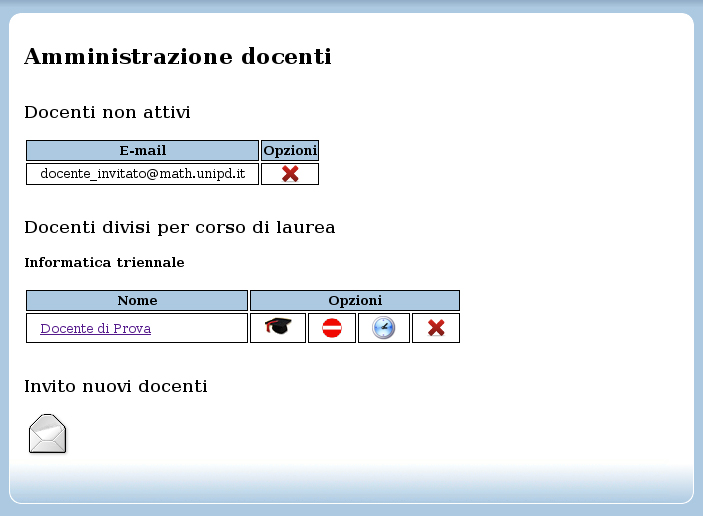
\includegraphics[scale=0.5]{images/amministrazione_docenti.jpg}\\
	\textbf{fig. 4.2.4.1} Pagina di gestione dei docenti\\
\end{center}
\bigskip

A seguire è presente una lista dei docenti già correttamente registrati all'interno del sistema, ma che non sono assegnati a nessun corso di laurea.
I docenti assegnati sono invece elencati e raggruppati per corso di laurea.
Per ogni docente è data la possibilità di:
\begin{itemize}
 \item consultare le informazioni relative ad un docente cliccando sul link presente sul suo nome.
 \item aggiungere il docente ad un altro corso di laurea seguendo il link `Gestione dei corsi di laurea associati`, caratterizzato dalla prima icona partendo da sinistra.
 \item aggiungere dei privilegi al docente selezionato, seguendo il link `Gestione dei privilegi`, il secondo partendo da sinistra: questa funzione è particolarmente utile se si rivelasse la necessità di avere un docente che affianchi la segreteria didattica nella parte amministrativa del sistema SIGEOL (di default, il presidente del CCS è già un docente con tali privilegi, ma potrebbe nascere la necessità di avere un altro docente con qualche privilegio amministrativo).
 \item gestire i vincoli temporali di indisponibilità del docente seguendo il link `Gestione dei vincoli e delle preferenze del docente`, caratterizzato dall'icona a forma di orologio.
 \item eliminare quel docente seguendo il link `Elimina definitivamente dal sistema`, caratterizzato dall'icona a forma di X rossa. Una finestra di popup chiederà conferma di tale azione. Tale azione non ha possibilità di essere annullata.
\end{itemize}

Le funzionalità di invito nuovo docente, di gestione dei corsi di laurea, di gestione dei privilegi e di gestione dei vincoli saranno illustrate dettagliatamente qui di seguito:
\newline \newline
\begin{large}\textbf{Invito di un docente:}\end{large}

\bigskip
\begin{center}
	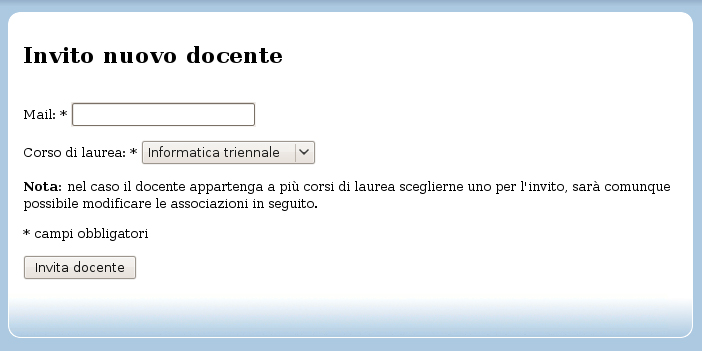
\includegraphics[scale=0.5]{images/invito_docenti.jpg}\\
	\textbf{fig. 4.2.5.1} Form di invito di un docente\\
\end{center}
\bigskip

Nella pagina di invito di un nuovo docente, come illustrato in figura 4.2.5.1, è sufficiente inserire l'indirizzo email a cui recapitare l'invito e, tramite menu a tendina, il corso di laurea per il quale il docente è richiesto.

Premendo il pulsante `Invita Docente` verrà automaticamente spedita un e-mail all'indirizzo specificato: tale e-mail conterrà delle brevi istruzioni che il docente dovrà seguire per completare la propria iscrizione al sistema SIGEOL.
Per ulteriori informazioni sulla procedura di attivazione dell'account di un docente si prega di consultare il documento \textsc{Manuale Utente Docente}.
\newline \newline
\begin{large}\textbf{Gestione dei corsi di laurea:}\end{large}

\bigskip
\begin{center}
	%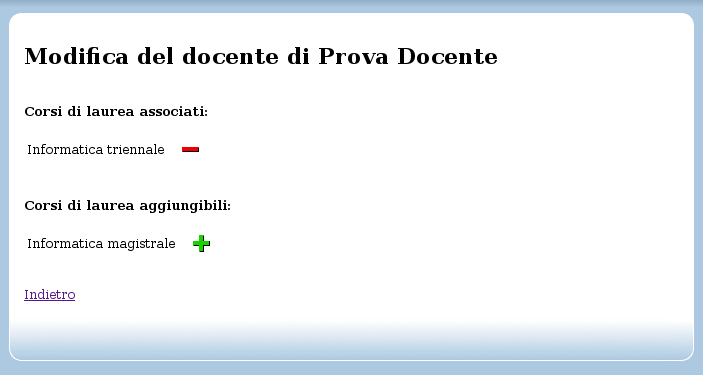
\includegraphics[scale=0.5]{images/gestione_corsi.jpg}\\
	\textbf{fig. 4.2.5.1} Pagina di gestione dei corsi di laurea\\
\end{center}
\bigskip

La pagina di gestione dei corsi di laurea per i docenti mostra innanzitutto una lista dei corsi di laurea per i quali il docente in esame è stato dichiarato disponibile. A fianco di ognuno di essi, è possibile seguire il link `Togli corso di laurea` per eliminare la disponibilità del docente ad essere assegnato ad un insegnamento di quel particolare corso di laurea. Tale link è identificabile da un icona a forma di - rossa.

A seguire, è presente una lista di tutti i corsi di laurea registrati al sistema SIGEOL: seguendo il link `Aggiungi corso di laurea`, caratterizzato dall'icona + verde, è possibile mettere a disposizione il docente in esame per quel determinato corso di laurea.
\newline \newline
\begin{large}\textbf{Gestione dei privilegi:}\end{large}

\bigskip
\begin{center}
	%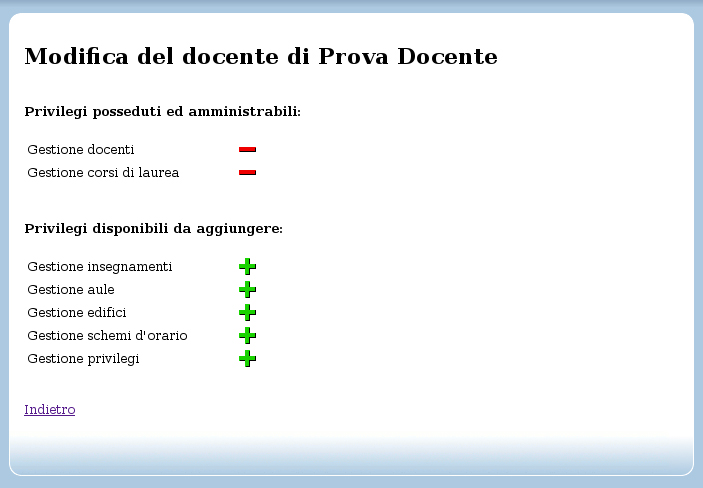
\includegraphics[scale=0.5]{images/gestione_privilegi.jpg}\\
	\textbf{fig. 4.2.5.1} Pagina di gestione dei privilegi\\
\end{center}
\bigskip

La pagina di gestione privilegi, come visibile in figura 4.2.5.1, permette di assegnare delle capacità amministrative al docente in esame. Questo può essere utile nel caso si voglia dare la possibilità di utilizzare le funzioni amministrative a qualche altro utente.

Un esempio dell'utilità di tale funzione è rappresentata dal presidente del CCS: si tratta infatti di un docente, ma con in più tutte le capacità amministrative tipiche della segreteria didattica.

Per aggiungere un dato privilegio a un docente, è sufficiente seguire il link `Aggiungi privilegio`, caratterizzato dall'icona - verde, presente a fianco di ogni tipologia di privilegio.

Al contrario, è anche possibile limitare le capacità di un determinato docente al qualche erano state precedentemente aggiunte. Per fare ciò è necessario seguire il link `Togli privilegio`, caratterizzato dall'icona + rossa presente a fianco di ogni privilegio che il docente in esame ha a disposizione.
\newline \newline
\begin{large}\textbf{Gestione dei vincoli temporali:}\end{large}

\bigskip
\begin{center}
	%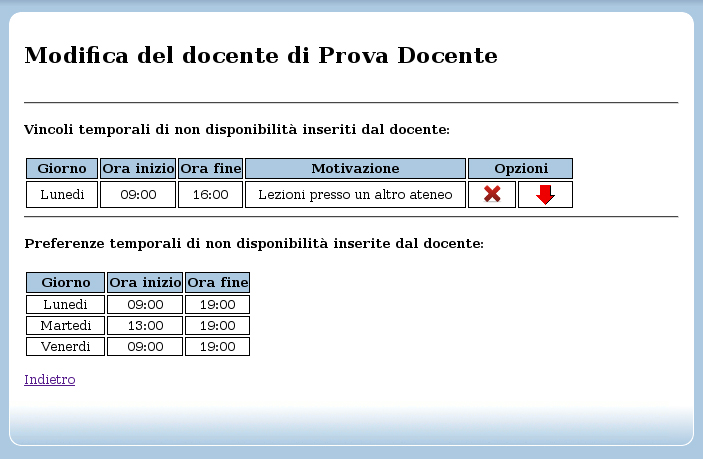
\includegraphics[scale=0.5]{images/gestione_vincoli_docenti.jpg}\\
	\textbf{fig. 4.2.5.1} Pagina di gestione dei vincoli temporali\\
\end{center}
\bigskip

La pagina di gestione dei vincoli temporali dei docenti, come visibile in figura 4.2.5.1, permette di monitorare i vincoli e le preferenze che i docenti hanno inserito nel sistema. Questo controllo è di vitale importanza perchè un numero troppo elevato di vincoli potrebbe impedire la generazione dell'orario delle lezioni, a causa delle troppe indisponibilità dichiarate dei docenti.

Questa pagina permette alla segreteria didattica, dopo aver valutato attentamente le varie motivazioni dei vincoli, di:
\begin{itemize}
 \item eliminare definitivamente il vincolo dal sistema, seguendo il link `Elimina definitivamente il vincolo`, caratterizzato dall'icona a forma di X rossa.
 \item trasformare il vincolo in una preferenza: in questo modo, il sistema di generazione dell'orario terrà lo stesso conto di questa non disponibilità, ma non sarà più costretto a rispettarla. In caso di necessità, potrà essere ignorata per rispettare vincoli più importanti in quanto preferenza e non più vincolo. La nuova preferenze generata da quest'operazione avrà priorità maggiore di tutte le preferenze preesistenti.
\end{itemize}
In entrambi i casi verrà mandata una notifica via e-mail dell'avvenuto cambiamento al docente interessato. Quest'ultimo potrà discutere personalmente con la segreteria le motivazioni della scelta e potrà accrdarsi per un eventuale rigenerazione dell'orario delle lezioni.
\subsubsection{Cambio Password}
La pagina di cambio password permette semplicemente di modificare la password del proprio \underline{account}. E' raggiungibile seguendo il link `Cambio password` presente nella barra laterale.

La procedura è particolarmente semplice: è sufficiente inserire esattamente la password vecchia, inserire la nuova password e la sua conferma e, per finire, premere il pulsante `Cambia Password`, come illustrato in figura 4.2.4.1.

\bigskip
\begin{center}
	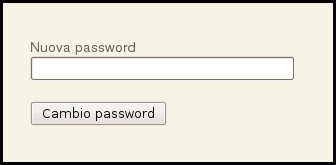
\includegraphics[scale=0.5]{images/cambio_password.jpg}\\
	\textbf{fig. 4.2.4.1} Form di cambio password\\
\end{center}
\bigskip

\subsubsection{Gestione dell'orario delle lezioni}
La pagina di gestione dell'orario delle lezioni, raggiungibile seguendo il link `Orario` presente nella barra laterale, permette alla segreteria didattica di far calcolare al sistema SIGEOL la miglior soluzione possibile di orario tenendo conto di tutti i dati che sono stati inseriti nelle precedenti fasi.

Tale pagina, come visibile in figura 4.2.8.1, fornisce una visione d'insieme dei vari corsi di laurea gestiti dal sistema SIGEOL, raggruppati per anno accademico e quindi per periodo.

\bigskip
\begin{center}
	%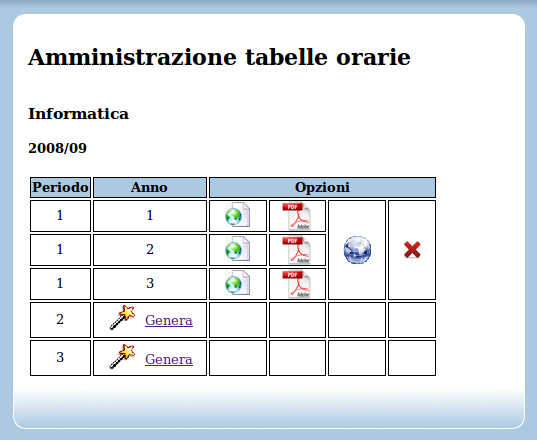
\includegraphics[scale=0.5]{images/amministrazione_orario.jpg}\\
	\textbf{fig. 4.2.8.1} Pagina di gestione degli orari delle lezioni\\
\end{center}
\bigskip

Per ogni combinazione di periodo, anno accademico e corso di laurea è possibile:
\begin{itemize}
 \item generare l'orario delle lezioni seguendo il link ``
 \item se l'orario è già stato generato dal sistema, è possibile renderlo pubblico
 \item se l'orario è già stato generato e non è più necessario, è possibile eliminarlo
\end{itemize}
Il calcolo dello schema d'orario non è istantaneo, ma potrà richiedere svariati minuti, in base anche alla complessità e al numero di dati inseriti.
La generazione dell'orario è indipendente dal sito internet del progetto: non è quindi necessario attendere la fine dei calcoli sulla pagina di generazione, ma è possibile compiere altre azioni o addirittura spegnere il calcolatore da cui è stata lanciata la richiesta.

Al termine del calcolo algoritmico, l'orario sarà reso disponibile nella pagina di gestione degli orari del progetto SIGEOL.

Si ricorda che allo scadere della data limite di inserimento dei vincoli dei docenti impostata in fase di creazione dell'orario (vedi sezione seguente) verrà automaticamente generato un orario di lezione, senza alcuna richiesta da parte della segreteria didattica. Potrà comunque essere generato nuovamente l'orario delle lezioni in seguito, per esempio dopo l'inserimento di nuove aule o di nuovi vincoli.

Verrà qui di seguito illustrata nel dettaglio la funzionalità di generazione dell'orario delle lezioni:
\newline \newline
\begin{large}\textbf{Generazione dell'orario delle lezioni:}\end{large}

\bigskip
\begin{center}
	%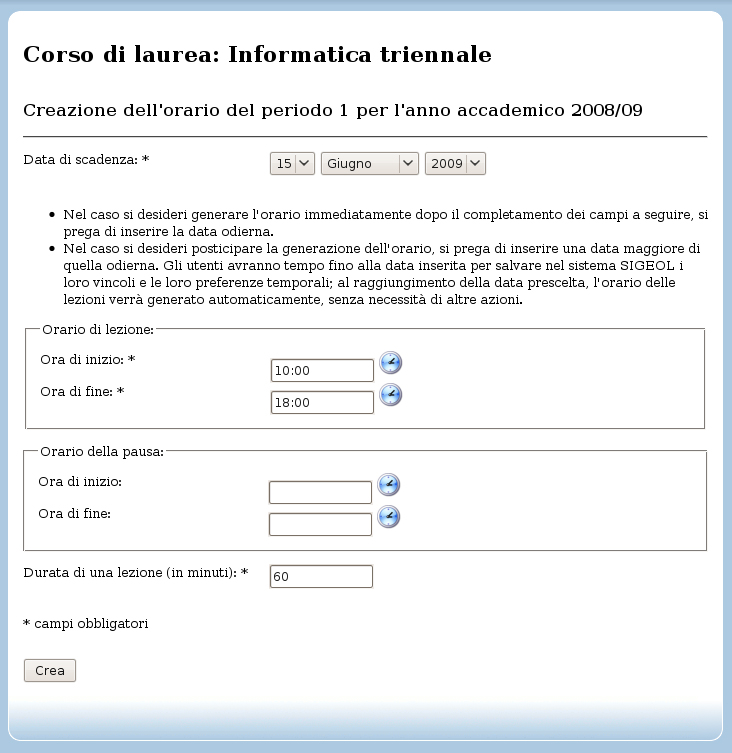
\includegraphics[scale=0.5]{images/generazione_orario.jpg}\\
	\textbf{fig. 4.2.8.2} Pagina di generazione dell'orario delle lezioni\\
\end{center}
\bigskip

La pagina di creazione di un nuovo orario delle lezioni, come visibile in figura 4.2.8.2, permette di lanciare la generazione di un orario per il corso di laurea e per il periodo prescelti.
Per la creazione dell'orario è necessario inserire i seguenti dati:
\begin{itemize}
 \item Data di scadenza: è la data in cui verrà generaro l'orario. Se si inserisce la data odierna, la generazione dell'orario viene lanciata immediatamente. Se nello stesso momento sono in fase di generazione altri orari di altri corsi di laurea, il sistema SIGEOL accoderà automaticamente la generazione del nuovo orario e la eseguirà il prima possibile. Se invece la data scelta è maggiore di quella odierna, il sistema schedulerà la generazione a quella data e la lancerà automaticamente: nel frattempo i docenti potranno inserire i loro vincoli e le loro preferenze di indisponibilità, e la segreteria potrà completare l'inserimento nel sistema di tutti i dati relativi agli edifici, alle aule, agli insegnamenti, ecc...
 \item Orario delle lezioni - ora di inizio: è l'ora in cui si vuole far iniziare la prima lezione di ogni giorno. L'algoritmo di calcolo dell'orario non potrà categoricamente inserire lezioni prima di quest'orario.
 \item Orario delle lezioni - ora di fine: è l'ora in cui si vuole far finire l'ultima lezione di ogni giorno. L'algoritmo di calcolo dell'orario non potrà categoricamente inserire lezioni dopo di quest'orario.
 \item Orario della pausa - ora di inizio: è l'ora in cui si vuole far cominciare la pausa, per dividere ogni giorno le lezioni in 2 blocchi.
 \item Orario della pausa - ora di fine: è l'ora in cui si vuole far finire la pausa. La pausa è facoltativa, ma nel caso di inserimento di un orario di inizio e di un orario di fine pausa l'algoritmo non potrà assolutamente assegnare delle lezioni nel periodo in cui è stata impostata la pausa.
 \item Durata di una lezione: inserire la durata, in minuti, di una lezione per quel determinato corso di laurea, comprensiva dell'eventuale pausa tra una lezione e la successiva.
\end{itemize}
Gli inserimento degli orari possono essere fatti sia in modo manuale (in tal caso l'orario va inserito nel formato HH:MM) sia in modo grafico, cliccando sull'icona dell'orologio.
La durata in minuti di una lezione deve essere invece scritta manualmente, e l'intervallo temporale tra ora di inizio delle lezioni e ora di fine deve essere un suo multiplo.

Dopo aver inserito tutti i dati richiesti, è sufficiente premere il bottone 'Crea' per lanciare o schedulare la generazione dell'orario delle lezioni per il corso di laurea e il periodo in esame.

Una volta che l'algoritmo di generazione dell'orario ha completato i suoi calcoli, si possono presentare 2 situazioni:
\begin{itemize}
 \item l'orario è stato generato correttamente: in questo caso, nella pagina di gestione degli orari è possibile utilizzare il link 'Pubblica' per rendere pubblico e consultabile l'orario delle lezioni. Se l'orario è stato generato, significa che nessuno dei vincoli registrati nel sistema SIGEOL è stato violato. Se qualche preferenza di qualche docente è stata invece non rispettata, una e-mail verrà mandata al docente in oggetto comunicando gli orari dell'insegnamento toccato da questo fatto. Il docente potrà eventualmente discutere personalmente un eventuale rigenerazione dell'orario se dovessero sorgere gravi problematiche. In qualsiasi caso, non potrà comunque essere pubblicato un orario delle lezioni che non rispetti tutti i vincoli di indisponibilità dei docenti e delle aule.
 \item nello sfortunato caso invece che l'algoritmo di calcolo non riesca a generare un orario, verrà immediatamente mandata una e-mail alla segreteria didattica consigliando di:
	\begin{enumerate}
	 \item controllare i vincoli dei docenti segnalati nella e-mail: tali docenti potrebbero possedere troppi vincoli, tali da non permettere la generazione di un orario. La segreteria potrà in questo caso eliminare o trasformare in preferenza uno o più vincoli di quel docente.
	 \item Aumentare la durata giornaliera delle lezioni
	 \item Aumentare il numero di aule a disposizione del corso di laurea
	 \item Controllare i vincoli temporali delle aule segnalate all'interno della e-mail.
	\end{enumerate}
  Una volta controllati i punti appena elencati e fatte le opportune modifiche, la segreteria didattica dovrà provvedere alla rigenerazione dell'orario.
\end{itemize}
\subsection{Errori probabili e cause possibili}
L'inserimento dei dati nelle varie form da parte della segreteria didattica è seguito passo passo dal sistema SIGEOL: ogni dato è controllato e validato prima di essere salvato in modo persistente.

E' pertanto difficile, se non impossibile, inserire dati errati senza che questo venga segnalato.
La segnalazione degli errori avverrà in seguito alla pressione del pulsante di invio dei dati: verrà quindi visualizzata nuovamente la form da cui si era partiti, con in più la segnalazione dell'errore. Sarà quindi sufficiente correggere il dato che ha generato l'errore e premere nuovamente il pulsante di invio dei dati (che potrà essere `Salva`, `Salva Modifiche` o altro, in base alla form su cui si sta lavorando).

Per non andare incontro a segnalazioni continue di errori è necessario seguire le linee guida indicate nella sezione `Azioni richieste - permesse` del presente documento, di volta in volta consultando la sottosezione relativa alla funzionalità che si sta usando.

Oltre a segnalazioni per inserimenti errati o campi dato non completati, è possibile che si verifichino errori più gravi per cause non dipendenti dall'utente che sta usando il sistema in quel momento, dovuti per esempio all'infrastruttura di rete o a problemi hardware dei personal computer impiegati.
Per una lista completa di tali errori, per le possibili cause e per le eventuali soluzioni si prega di consultare la sezione `Messaggi di errore e loro significato` presente in appendice al presente documento.
\newpage
\section{Appendice}
\subsection{Messaggi di errore e loro significato}
\subsection{Glossario}
\flushleft \Huge A \bigskip
\hrule
\smallskip
\normalsize
\begin{description}
	\item[Account:] insieme di funzionalità, strumenti e contenuti attribuiti ad un utente in determinati contesti operativi. In informatica, attraverso il meccanismo dell'account, il sistema mette a disposizione dell'utente un ambiente con contenuti e funzionalità personalizzabili, oltre ad un conveniente grado di isolamento dalle altre utenze parallele.
\end{description}
\bigskip
\Huge B \bigskip
\hrule
\smallskip
\normalsize
\begin{description}
	\item[Browser:] software che consente agli utenti di visualizzare e interagire con testi, immagini e altre informazioni, tipicamente contenute in una pagina web di un sito. Il browser è in grado di interpretare il codice HTML (e più recentemente XHTML) e visualizzarlo in forma di ipertesto. L'HTML è il codice col quale la maggioranza delle pagine web nel mondo sono composte: il web browser consente perciò la navigazione nel web.
\end{description}
\bigskip
\Huge L \bigskip
\hrule
\smallskip
\normalsize
\begin{description}
	\item[Link:] letteralmente indica un collegamento. In informatica è usato per indicare l'indirizzo web di una risorsa.
	\item[Login:] termine inglese per indicare la procedura di accesso ad un sistema o un'applicazione informatica.
	\item[Logout:] termine inglese per indicare la procedura di uscita da un sistema o un'applicazione informatica.
\end{description}
\bigskip
\Huge P \bigskip
\hrule
\smallskip
\normalsize
\begin{description}
	\item[Pdf:] il Portable Document Format, comunemente abbreviato Pdf, è un formato di file basato su un linguaggio di descrizione di pagina sviluppato da Adobe per rappresentare documenti in modo indipendente dall'hardware e dal software utilizzati per generarli o per visualizzarli. Ogni documento redatto dal team QuiXoft viene esportato in questo formato.
\end{description}
\bigskip
\Huge S \bigskip
\hrule
\smallskip
\normalsize
\begin{description}
	\item[Screenshot:] termine inglese (da screen, schermo, e shot, scatto fotografico) che indica l'istantanea di ciò che visualizzato in un determinato istante sullo schermo di un elaboratore.
\end{description}
\bigskip
\Huge T \bigskip
\hrule
\smallskip
\normalsize
\begin{description}
	\item[Template:] documento o programma dove, come in un foglio semicompilato cartaceo, su una struttura generica o standard esistono spazi temporaneamente "bianchi" da riempire successivamente.
\end{description}
\bigskip
\Huge W \bigskip
\hrule
\smallskip
\normalsize
\begin{description}
	\item[World Wide Web:] termine di origine inglese, in sigla WWW e spesso abbreviato in Web, è uno dei servizi di Internet, la più grande rete ad accesso pubblico di computer mai realizzata. In particolare il Web è, assieme alla posta elettronica, il servizio di Internet più utilizzato e conosciuto.
\end{description}
\modifiche
\end{document}
